%%%%%%%%%%%%%%%%%%%%%%%%%%%%%%%%%%%%%%%%%%%%%%%%%%%%%%%%%%%%%%%%%%%%%%%%%%%%%%%%
%% Plantilla de memoria en LaTeX para la ETSIT - Universidad Rey Juan Carlos
%%
%% Por Gregorio Robles <grex arroba gsyc.urjc.es>
%%     Grupo de Sistemas y Comunicaciones
%%     Escuela Técnica Superior de Ingenieros de Telecomunicación
%%     Universidad Rey Juan Carlos
%% (muchas ideas tomadas de Internet, colegas del GSyC, antiguos alumnos...
%%  etc. Muchas gracias a todos)
%%
%% La última versión de esta plantilla está siempre disponible en:
%%     https://github.com/gregoriorobles/plantilla-memoria
%%
%% Para obtener PDF, ejecuta en la shell:
%%   make
%% (las imágenes deben ir en PNG o JPG)

%%%%%%%%%%%%%%%%%%%%%%%%%%%%%%%%%%%%%%%%%%%%%%%%%%%%%%%%%%%%%%%%%%%%%%%%%%%%%%%%

\documentclass[a4paper, 12pt, english]{book}
\usepackage[T1]{fontenc}


\usepackage[a4paper, left=2.5cm, right=2.5cm, top=3cm, bottom=3cm]{geometry}
\usepackage{times}
%\usepackage[spanish]{babel} % Comenta esta línea si tu memoria es en inglés
\usepackage{url}
%\usepackage[dvipdfm]{graphicx}
\usepackage{graphicx}
\usepackage{float}  %% H para posicionar figuras
\usepackage[nottoc, notlot, notlof, notindex]{tocbibind} %% Opciones de índice
\usepackage{latexsym}  %% Logo LaTeX

\usepackage[T1]{fontenc}
\usepackage{selinput}
\SelectInputMappings{%
  aacute={á},
  ntilde={ñ},
  Euro={€}
}
\usepackage{babel}

\usepackage{hyperref}

\title{Memoria del Proyecto}
\author{Ismael Slimane Zubillaga}

\renewcommand{\baselinestretch}{1.5}  %% Interlineado

\begin{document}

\renewcommand{\refname}{Bibliografía}  %% Renombrando
\renewcommand{\appendixname}{Apéndice}

%%%%%%%%%%%%%%%%%%%%%%%%%%%%%%%%%%%%%%%%%%%%%%%%%%%%%%%%%%%%%%%%%%%%%%%%%%%%%%%%
% PORTADA

\begin{titlepage}
\begin{center}
\begin{tabular}[c]{c c}
%\includegraphics[bb=0 0 194 352, scale=0.25]{logo} &

\includegraphics[scale=0.25]{img/logo_vect.png} &
\begin{tabular}[b]{l}
\Huge
\textsf{UNIVERSIDAD} \\
\Huge
\textsf{REY JUAN CARLOS} \\
\end{tabular}
\\
\end{tabular}

\vspace{3cm}

\Large
INGENIERÍA EN TECNOLOGÍAS DE LA TELECOMUNICACIÓN

\vspace{0.4cm}

\large
Curso Académico 2017/2018

\vspace{0.8cm}

Trabajo Fin de Grado/Máster

\vspace{2.5cm}

\LARGE
SAKURA
\vspace{0.1cm}

\LARGE
ANGULAR 4 - ELASTICSEARCH - DASHBOARD INTERFACE

\vspace{4cm}

\large
Autor : Ismael Slimane Zubillaga \\
Tutor : Dr. Jesús M. González-Barahona
\end{center}
\end{titlepage}

\newpage
\mbox{}
\thispagestyle{empty} % para que no se numere esta pagina


%%%%%%%%%%%%%%%%%%%%%%%%%%%%%%%%%%%%%%%%%%%%%%%%%%%%%%%%%%%%%%%%%%%%%%%%%%%%%%%%
%%%% Para firmar
\clearpage
\pagenumbering{gobble}
\chapter*{}

\vspace{-4cm}
\begin{center}
\LARGE
\textbf{Trabajo Fin de Grado/Máster}

\vspace{1cm}
\large
Título del Trabajo con Letras Capitales para Sustantivos y Adjetivos

\vspace{1cm}
\large
\textbf{Autor :} Nombre del Alumno/a \\
\textbf{Tutor :} Dr. Gregorio Robles Martínez

\end{center}

\vspace{1cm}
La defensa del presente Proyecto Fin de Carrera se realizó el día \qquad$\;\,$ de \qquad\qquad\qquad\qquad \newline de 20XX, siendo calificada por el siguiente tribunal:


\vspace{0.5cm}
\textbf{Presidente:}

\vspace{1.2cm}
\textbf{Secretario:}

\vspace{1.2cm}
\textbf{Vocal:}


\vspace{1.2cm}
y habiendo obtenido la siguiente calificación:

\vspace{1cm}
\textbf{Calificación:}


\vspace{1cm}
\begin{flushright}
Fuenlabrada, a \qquad$\;\,$ de \qquad\qquad\qquad\qquad de 20XX
\end{flushright}

%%%%%%%%%%%%%%%%%%%%%%%%%%%%%%%%%%%%%%%%%%%%%%%%%%%%%%%%%%%%%%%%%%%%%%%%%%%%%%%%
%%%% Dedicatoria

\chapter*{}
\pagenumbering{Roman} % para comenzar la numeracion de paginas en numeros romanos
\begin{flushright}
\textit{Dedicado a \\
mi familia / mi abuelo / mi abuela}
\end{flushright}

%%%%%%%%%%%%%%%%%%%%%%%%%%%%%%%%%%%%%%%%%%%%%%%%%%%%%%%%%%%%%%%%%%%%%%%%%%%%%%%%
%%%% Agradecimientos

\chapter*{Agradecimientos}
%\addcontentsline{toc}{chapter}{Agradecimientos} % si queremos que aparezca en el índice
\markboth{AGRADECIMIENTOS}{AGRADECIMIENTOS} % encabezado

Aquí vienen los agradecimientos\ldots Aunque está bien acordarse de la pareja, no hay que olvidarse de dar las gracias a tu madre, que aunque a veces no lo parezca disfrutará tanto de tus logros como tú\ldots
Además, la pareja quizás no sea para siempre, pero tu madre sí.

%%%%%%%%%%%%%%%%%%%%%%%%%%%%%%%%%%%%%%%%%%%%%%%%%%%%%%%%%%%%%%%%%%%%%%%%%%%%%%%%
%%%% Resumen

\chapter*{Resumen}
%\addcontentsline{toc}{chapter}{Resumen} % si queremos que aparezca en el índice
\markboth{RESUMEN}{RESUMEN} % encabezado

Aquí viene un resumen del proyecto. Ha de constar de tres o cuatro párrafos, donde se presente de manera clara y concisa de qué va el proyecto.
Han de quedar respondidas las siguientes preguntas:

\begin{itemize}
  \item ¿De qué va este proyecto? ¿Cuál es su objetivo principal?
  \item ¿Cómo se ha realizado? ¿Qué tecnologías están involucradas?
  \item ¿En qué contexto se ha realizado el proyecto? ¿Es un proyecto
dentro de un marco general?
\end{itemize}

Lo mejor es escribir el resumen al final.

%%%%%%%%%%%%%%%%%%%%%%%%%%%%%%%%%%%%%%%%%%%%%%%%%%%%%%%%%%%%%%%%%%%%%%%%%%%%%%%%
%%%% Resumen en inglés

\chapter*{Summary}
%\addcontentsline{toc}{chapter}{Summary} % si queremos que aparezca en el índice
\markboth{SUMMARY}{SUMMARY} % encabezado

Here comes a translation of the ``Resumen'' into English. Please, double check it for correct grammar and spelling.
As it is the translation of the ``Resumen'', which is supposed to be written at the end, this as well should be filled out
just before submitting.


%%%%%%%%%%%%%%%%%%%%%%%%%%%%%%%%%%%%%%%%%%%%%%%%%%%%%%%%%%%%%%%%%%%%%%%%%%%%%%%%
%%%%%%%%%%%%%%%%%%%%%%%%%%%%%%%%%%%%%%%%%%%%%%%%%%%%%%%%%%%%%%%%%%%%%%%%%%%%%%%%
% ÍNDICES %
%%%%%%%%%%%%%%%%%%%%%%%%%%%%%%%%%%%%%%%%%%%%%%%%%%%%%%%%%%%%%%%%%%%%%%%%%%%%%%%%

% Las buenas noticias es que los índices se generan automáticamente.
% Lo único que tienes que hacer es elegir cuáles quieren que se generen,
% y comentar/descomentar esa instrucción de LaTeX.

%%%% Índice de contenidos
\tableofcontents
%%%% Índice de figuras
\cleardoublepage
%\addcontentsline{toc}{chapter}{Lista de figuras} % para que aparezca en el indice de contenidos
\listoffigures % indice de figuras
%%%% Índice de tablas
%\cleardoublepage
%\addcontentsline{toc}{chapter}{Lista de tablas} % para que aparezca en el indice de contenidos
%\listoftables % indice de tablas


%%%%%%%%%%%%%%%%%%%%%%%%%%%%%%%%%%%%%%%%%%%%%%%%%%%%%%%%%%%%%%%%%%%%%%%%%%%%%%%%
%%%%%%%%%%%%%%%%%%%%%%%%%%%%%%%%%%%%%%%%%%%%%%%%%%%%%%%%%%%%%%%%%%%%%%%%%%%%%%%%
% INTRODUCCIÓN %
%%%%%%%%%%%%%%%%%%%%%%%%%%%%%%%%%%%%%%%%%%%%%%%%%%%%%%%%%%%%%%%%%%%%%%%%%%%%%%%%

\cleardoublepage
\chapter{Introducción}
\label{sec:intro} % etiqueta para poder referenciar luego en el texto con ~\ref{sec:intro}
\pagenumbering{arabic} % para empezar la numeración de página con números

En este capítulo se introduce el proyeto. Debería tener información general sobre el mismo, dando la información sobre el contexto en el que se ha desarrollado.

No te olvides de echarle un ojo a la página con los cinco errores de escritura más frecuentes\footnote{\url{http://www.tallerdeescritores.com/errores-de-escritura-frecuentes}}.

Aconsejo a todo el mundo que mire y se inspire en memorias pasadas. Las mías están todas almacenadas en mi web del GSyC\footnote{\url{https://gsyc.urjc.es/~grex/pfcs/}}.

\section{Descripción del Problema}
\label{sec:descripcion}

%Esto es una sección, que es una estructura menor que un capítulo.

%Por cierto, a veces me comentáis que no os compila por las tildes.
%Eso es un problema de codificación.
%Cambiad de ``UTF-8'' a ``ISO-Latin-1'' (o vicecersa) y funcionará.

%\subsection{Estilo}
%\label{subsec:estilo}

%Recomiendo leer los consejos prácticos sobre LaTeX de Diomidos
%Spinellis\footnote{\url{https://github.com/dspinellis/latex-advice}}.

%Sobre el uso de las comas\footnote{\url{http://narrativabreve.com/2015/02/opiniones-de-un-corrector-de-estilo-11-%recetas-para-escribir-correctamente-la-coma.html}}

%A continuación, viene una figura, la Figura~\ref{figura:foro_hilos}.
%Observarás que el texto dentro del a referencia es el identificador de la figura (que se corresponden con el ``label'' dentro de la misma).
%También habrás tomado nota de cómo se ponen las ``comillas dobles'' para que se muestren correctamente.
%Volviendo a las referencias, nota que al compilar, la primera vez se crea un diccionario con las referencias, y en la segunda compilación se ``rellenan'' estas referencias.
%Por eso hay que compilar dos veces.

% \begin{figure}
%    \centering
%    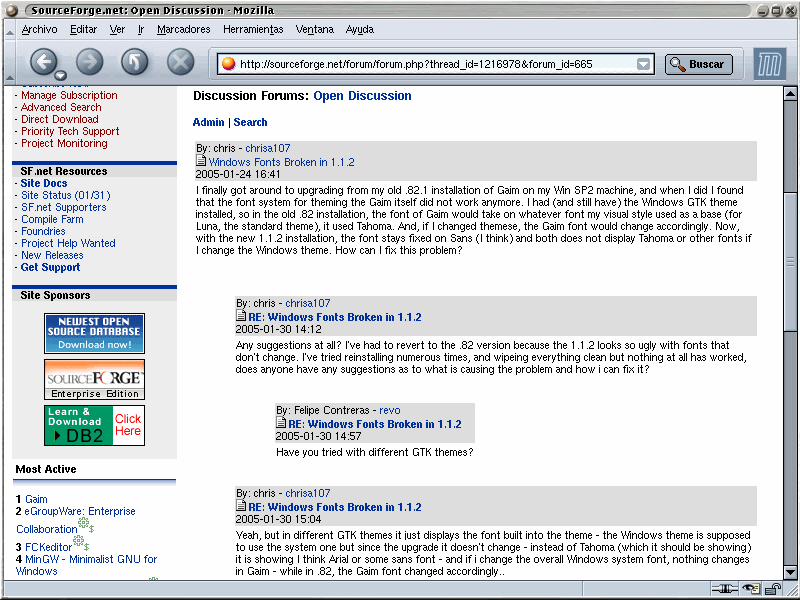
\includegraphics[bb=0 0 800 600, width=12cm, keepaspectratio]{img/foro1}
%    \caption{Página con enlaces a hilos}
%    \label{figura:foro_hilos}
% \end{figure}

%{\footnotesize
%\begin{verbatim}
%    From gaurav at gold-solutions.co.uk  Fri Jan 14 14:51:11 2005
%    From: gaurav at gold-solutions.co.uk (gaurav_gold)
%    Date: Fri Jan 14 19:25:51 2005
%    Subject: [Mailman-Users] mailman issues
%    Message-ID: <003c01c4fa40$1d99b4c0$94592252@gaurav7klgnyif>

%    Dear Sir/Madam,
%    How can people reply to the mailing list?  How do i turn off
%    this feature? How can i also enable a feature where if someone
%    replies the newsletter the email gets deleted?
%    Thanks

%    From msapiro at value.net  Fri Jan 14 19:48:51 2005
%    From: msapiro at value.net (Mark Sapiro)
%%    Date: Fri Jan 14 19:49:04 2005
 %   Subject: [Mailman-Users] mailman issues
%    In-Reply-To: <003c01c4fa40$1d99b4c0$94592252@gaurav7klgnyif>
%    Message-ID: <PC173020050114104851057801b04d55@msapiro>

%%    gaurav_gold wrote:
%    >How can people reply to the mailing list?  How do i turn off
%    this feature? How can i also enable a feature where if someone
%    replies the newsletter the email gets deleted?

%    See the FAQ
%    >Mailman FAQ: http://www.python.org/cgi-bin/faqw-mm.py
%    article 3.11
%\end{verbatim}
%}

\section{Objetivo Principal y Estructura}
\label{sec:objetivo}

En esta sección se debería introducir la esctura de la memoria. Así:

\begin{itemize}
  \item En el primer capítulo se hace una intro al proyecto.

  \item En el capítulo~\ref{chap:objetivos} (ojo, otra referencia automática) se muestran los objetivos del proyecto.

  \item A continuación se presenta el estado del arte.

  \item \ldots
\end{itemize}

\section{Disponibilidad del Software}
\label{sec:objetivo}


%%%%%%%%%%%%%%%%%%%%%%%%%%%%%%%%%%%%%%%%%%%%%%%%%%%%%%%%%%%%%%%%%%%%%%%%%%%%%%%%
%%%%%%%%%%%%%%%%%%%%%%%%%%%%%%%%%%%%%%%%%%%%%%%%%%%%%%%%%%%%%%%%%%%%%%%%%%%%%%%%
% OBJETIVOS %
%%%%%%%%%%%%%%%%%%%%%%%%%%%%%%%%%%%%%%%%%%%%%%%%%%%%%%%%%%%%%%%%%%%%%%%%%%%%%%%%

\cleardoublepage % empezamos en página impar
\chapter{State of Art} % título del capítulo (se muestra)
\label{chap:state-of-art} % identificador del capítulo (no se muestra, es para poder referenciarlo)

\section{ElasticSearch} % título de sección (se muestra)
\label{sec:elasticsearch} % identificador de sección (no se muestra, es para poder referenciarla)

\textit{\textbf{Elasticsearch}} is an open-source, \textit{broadly-distributable}, \textit{readily-scalable}, \textit{enterprise-grade} search engine based on Lucene\footnote{\url{https://en.wikipedia.org/wiki/Apache\_Lucene}}. It provides a distributed, multitenant-capable full-text search engine with an HTTP web interface and schema-free JSON documents.

\subsection{History}
\label{subsec:elasticsearch-history}
\textbf{Shay Banon} created the precursor to Elasticsearch, called \textit{Compass}, in 2004. While thinking about the third version of Compass he realized that it would be necessary to rewrite big parts of Compass to "create a scalable search solution". So he created "a solution built from the ground up to be distributed" and used a common interface, \textit{JSON} over \textit{HTTP}, suitable for programming languages other than \textit{Java} as well. Shay Banon released the first version of Elasticsearch in February 2010.

\subsection{Main Concepts}
\label{subsec:elasticsearch-main-concepts}

All the following concepts definitions are extracted from the Elasticsearch documentation web page\footnote{\url{https://www.elastic.co/guide/en/elasticsearch/reference/current/_basic_concepts.html}}.

\begin{itemize}
    \item \textbf{Near Realtime (NRT)}:
        Elasticsearch is a near real time search platform. What this means is there is a slight latency (normally one second) from the time you index a document until the time it becomes searchable.
    \item \textbf{Index}:
        An index is a collection of documents that have somewhat similar characteristics. For example, you can have an index for customer data, another index for a product catalog, and yet another index for order data. An index is identified by a name (that must be all lowercase) and this name is used to refer to the index when performing indexing, search, update, and delete operations against the documents in it.
        In a single cluster, you can define as many indexes as you want.
    \item \textbf{Shards & Replicas}:
        An index can potentially store a large amount of data that can exceed the hardware limits of a single node.

        To solve this problem, Elasticsearch provides the ability to subdivide your index into multiple pieces called \textbf{shards}. When you create an index, you can simply define the number of shards that you want. Each shard is in itself a fully-functional and independent "index" that can be hosted on any node in the cluster.

        In a network/cloud environment where failures can be expected anytime, it is very useful and highly recommended to have a failover mechanism in case a shard/node somehow goes offline or disappears for whatever reason. To this end, Elasticsearch allows you to make one or more copies of your index’s shards into what are called \textit{replica shards}, or \textbf{replicas} for short.
    \item \textbf{Type}:
        A type in Elasticsearch represents a class of similar documents. A type consists of a \textit{name}—such as user or blogpost—and a \textit{mapping}. The \textit{mapping}, like a database schema, describes the fields or properties that documents of that type may have, the datatype of each field—such as string, integer, or date—and how those fields should be indexed and stored by \textit{Lucene}.
    \item \textbf{Document}:
        A document is a basic unit of information that can be indexed. For example, you can have a document for a single customer, another document for a single product, and yet another for a single order. This document is expressed in JSON (JavaScript Object Notation) which is an ubiquitous internet data interchange format.
    \item \textbf{Node}:
        A node is a single server that is part of your cluster, stores your data, and participates in the cluster’s indexing and search capabilities.
    \item \textbf{Cluster}:
        A cluster is a collection of one or more nodes (servers) that together holds your entire data and provides federated indexing and search capabilities across all nodes.
\end{itemize}


\section{GitHub}
\label{sec:github}

Los objetivos específicos se pueden entender como las tareas en las que se ha desglosado el objetivo general.
Y, sí, también vienen en infinitivo.


\section{Webpack}
\label{sec:webpack}

\section{Angular 4}
\label{sec:angular4}

\section{TypeScript}
\label{sec:typeScript}

A mí me gusta que aquí pongáis una descripción de lo que os ha llevado realizar el trabajo.
Hay gente que añade un diagrama de GANTT.
Lo importante es que quede claro cuánto tiempo llevas (tiempo natural, p.ej., 6 meses) y a qué nivel de esfuerzo (p.ej., principalmente los fines de semana).


\section{JavaScript}
\label{sec:typeScript}

\section{Lodash}
\label{sec:flexbox}

\section{ChartJS}
\label{sec:chartJS}

\section{Canvas}
\label{sec:canvas}

\section{SASS}
\label{sec:sass}

\section{Flexbox}
\label{sec:flexbox}


%%%%%%%%%%%%%%%%%%%%%%%%%%%%%%%%%%%%%%%%%%%%%%%%%%%%%%%%%%%%%%%%%%%%%%%%%%%%%%%%
%%%%%%%%%%%%%%%%%%%%%%%%%%%%%%%%%%%%%%%%%%%%%%%%%%%%%%%%%%%%%%%%%%%%%%%%%%%%%%%%
% ESTADO DEL ARTE %
%%%%%%%%%%%%%%%%%%%%%%%%%%%%%%%%%%%%%%%%%%%%%%%%%%%%%%%%%%%%%%%%%%%%%%%%%%%%%%%%

%\cleardoublepage
%\chapter{Estado del arte}

%Descripción de las tecnologías que utilizas en tu trabajo.
%Con dos o tres párrafos por cada tecnología, vale.
%Se supone que aquí viene todo lo que no has hecho tú.

%Puedes citar libros, como el de Bonabeau et al. sobre procesos estigmérgicos~\cite{bonabeau:_swarm}. % Nota que el ~ añade un espacio en blanco, pero no deja que exista un salto de línea. Imprescindible ponerlo para las citas.

%También existe la posibilidad de poner notas al pie de página, por ejemplo, una para indicarte que visite la página de LibreSoft\footnote{\url{http://www.libresoft.es}}.

%\section{Sección 1}
%\label{sec:seccion1}

%Hemos hablado de cómo incluir figuras.
%Pero no hemos dicho nada de tablas.
%A mí me gustan las tablas.
%Mucho.
%Aquí un ejemplo de tabla, la Tabla~\ref{tabla:ejemplo}.

%\begin{table}
 %\begin{center}
%  \begin{tabular}{ | l | c | r |} % tenemos tres colummnas, la primera alineada a la izquierda (l), la segunda al centro (c) y la tercera a la derecha (r). El | indica que entre las columnas habrá una línea separadora.
%    \hline
%    1 & 2 & 3 \\ \hline % el hline nos da una línea vertical
%    4 & 5 & 6 \\ \hline
%    7 & 8 & 9 \\
%    \hline
%  \end{tabular}
%  \label{tabla:ejemplo}
%  \caption{Ejemplo de tabla}
% \end{center}
%\end{table}



%%%%%%%%%%%%%%%%%%%%%%%%%%%%%%%%%%%%%%%%%%%%%%%%%%%%%%%%%%%%%%%%%%%%%%%%%%%%%%%%
%%%%%%%%%%%%%%%%%%%%%%%%%%%%%%%%%%%%%%%%%%%%%%%%%%%%%%%%%%%%%%%%%%%%%%%%%%%%%%%%
% DISEÑO E IMPLEMENTACIÓN %
%%%%%%%%%%%%%%%%%%%%%%%%%%%%%%%%%%%%%%%%%%%%%%%%%%%%%%%%%%%%%%%%%%%%%%%%%%%%%%%%

\cleardoublepage
\chapter{Desarrollo}

Aquí viene todo lo que has hecho tú (tecnológicamente).
Puedes entrar hasta el detalle.
Es la parte más importante de la memoria, porque describe lo que has hecho tú.
Eso sí, normalmente aconsejo no poner código, sino diagramas.

\section{Metodología SCRUM}
\label{sec:scrum}

\section{Arquitectura general}
\label{sec:arquitectura}

Si tu proyecto es un software, siempre es bueno poner la arquitectura (que es cómo se estructura tu programa a ``vista de pájaro'').

Por ejemplo, puedes verlo en la figura~\ref{fig:arquitectura}.

\begin{figure}
  \centering
  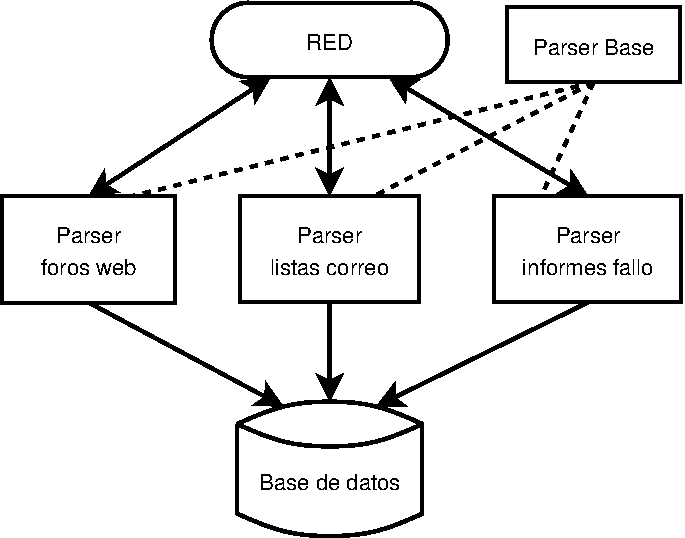
\includegraphics[width=9cm, keepaspectratio]{img/arquitectura}
  \caption{Estructura del parser básico}
  \label{fig:arquitectura}
\end{figure}

Si utilizas una base de datos, no te olvides de incluir también un diagrama de entidad-relación.


%%%%%%%%%%%%%%%%%%%%%%%%%%%%%%%%%%%%%%%%%%%%%%%%%%%%%%%%%%%%%%%%%%%%%%%%%%%%%%%%
%%%%%%%%%%%%%%%%%%%%%%%%%%%%%%%%%%%%%%%%%%%%%%%%%%%%%%%%%%%%%%%%%%%%%%%%%%%%%%%%
% RESULTADOS %
%%%%%%%%%%%%%%%%%%%%%%%%%%%%%%%%%%%%%%%%%%%%%%%%%%%%%%%%%%%%%%%%%%%%%%%%%%%%%%%%

\cleardoublepage
\chapter{Resultados}

En este capítulo se incluyen los resultados de tu trabajo fin de grado.

Si es una herramienta de análisis lo que has realizado, aquí puedes poner ejemplos de haberla utilizado para que se vea su utilidad.


%%%%%%%%%%%%%%%%%%%%%%%%%%%%%%%%%%%%%%%%%%%%%%%%%%%%%%%%%%%%%%%%%%%%%%%%%%%%%%%%
%%%%%%%%%%%%%%%%%%%%%%%%%%%%%%%%%%%%%%%%%%%%%%%%%%%%%%%%%%%%%%%%%%%%%%%%%%%%%%%%
% CONCLUSIONES %
%%%%%%%%%%%%%%%%%%%%%%%%%%%%%%%%%%%%%%%%%%%%%%%%%%%%%%%%%%%%%%%%%%%%%%%%%%%%%%%%

\cleardoublepage
\chapter{Conclusiones}
\label{chap:conclusiones}


\section{Consecución de objetivos}
\label{sec:consecucion-objetivos}

Esta sección es la sección espejo de las dos primeras del capítulo de objetivos, donde se planteaba el objetivo general y se elaboraban los específicos.

Es aquí donde hay que debatir qué se ha conseguido y qué no.
Cuando algo no se ha conseguido, se ha de justificar, en términos de qué problemas se han encontrado y qué medidas se han tomado para mitigar esos problemas.


\section{Aplicación de lo aprendido}
\label{sec:aplicacion}

Aquí viene lo que has aprendido durante el Grado/Máster y que has aplicado en el TFG/TFM. Una buena idea es poner las asignaturas más relacionadas y comentar en un párrafo los conocimientos y habilidades puestos en práctica.

\begin{enumerate}
  \item a
  \item b
\end{enumerate}


\section{Lecciones aprendidas}
\label{sec:lecciones_aprendidas}

Aquí viene lo que has aprendido en el Trabajo Fin de Grado/Máster.

\begin{enumerate}
  \item a
  \item b
\end{enumerate}


\section{Trabajos futuros}
\label{sec:trabajos_futuros}

Ningún software se termina, así que aquí vienen ideas y funcionalidades que estaría bien tener implementadas en el futuro.

Es un apartado que sirve para dar ideas de cara a futuros TFGs/TFMs.


%%%%%%%%%%%%%%%%%%%%%%%%%%%%%%%%%%%%%%%%%%%%%%%%%%%%%%%%%%%%%%%%%%%%%%%%%%%%%%%%
%%%%%%%%%%%%%%%%%%%%%%%%%%%%%%%%%%%%%%%%%%%%%%%%%%%%%%%%%%%%%%%%%%%%%%%%%%%%%%%%
% APÉNDICE(S) %
%%%%%%%%%%%%%%%%%%%%%%%%%%%%%%%%%%%%%%%%%%%%%%%%%%%%%%%%%%%%%%%%%%%%%%%%%%%%%%%%

\cleardoublepage
\appendix
\chapter{Manual de usuario}
\label{app:manual}


%%%%%%%%%%%%%%%%%%%%%%%%%%%%%%%%%%%%%%%%%%%%%%%%%%%%%%%%%%%%%%%%%%%%%%%%%%%%%%%%
%%%%%%%%%%%%%%%%%%%%%%%%%%%%%%%%%%%%%%%%%%%%%%%%%%%%%%%%%%%%%%%%%%%%%%%%%%%%%%%%
% BIBLIOGRAFIA %
%%%%%%%%%%%%%%%%%%%%%%%%%%%%%%%%%%%%%%%%%%%%%%%%%%%%%%%%%%%%%%%%%%%%%%%%%%%%%%%%

\cleardoublepage

% Las siguientes dos instrucciones es todo lo que necesitas
% para incluir las citas en la memoria
\bibliographystyle{abbrv}
\bibliography{memoria}  % memoria.bib es el nombre del fichero que contiene
% las referencias bibliográficas. Abre ese fichero y mira el formato que tiene,
% que se conoce como BibTeX. Hay muchos sitios que exportan referencias en
% formato BibTeX. Prueba a buscar en http://scholar.google.com por referencias
% y verás que lo puedes hacer de manera sencilla.
% Más información:
% http://texblog.org/2014/04/22/using-google-scholar-to-download-bibtex-citations/

\end{document}
